%%%% INF8225 Final Report: Graph Neural Networks for Fake News Detection

\documentclass{article}
\pdfpagewidth=8.5in
\pdfpageheight=11in
\usepackage{ijcai19}

\usepackage{times}
\usepackage{soul}
\usepackage{url}
\usepackage[hidelinks]{hyperref}
\usepackage[utf8]{inputenc}
\usepackage[small]{caption}
\usepackage{graphicx}
\usepackage{amsmath}
\usepackage{booktabs}
\urlstyle{same}

\title{Graph Neural Networks for Fake News Detection}

\author{
Ely Cheikh Abass\and
Omar Benzekri\and
Anis Abdeladim\\
\affiliations
Department of Computer Engineering and Software Engineering, Polytechnique Montréal\\
%\emails
%ely.cheikh-abass@polymtl.ca, omar.benzekri@polymtl.ca, anis.abdeladim@polymtl.ca
}

\begin{document}

\maketitle

\begin{abstract}
This report explores the application of Graph Neural Networks (GNNs) to the task of fake news detection. We present a literature review, describe our theoretical and experimental approach, and analyze the effectiveness of various GNN architectures on a graph-structured misinformation dataset.
\end{abstract}

\section{Introduction}
% Brief overview of fake news detection
% Summary of past work (cite 2-3 papers briefly)
% Why GNNs? Transition into theoretical foundations

Fake news, often defined as low-quality or fabricated news intended to mislead readers, has emerged as a significant societal problem in the age of social media~\cite{Shu2017}. Online platforms enable the rapid and wide dissemination of misinformation, allowing fake news to reach millions of users with ease. The extensive spread of fake news can distort public opinion and undermine trust in institutions, leading to harmful real-world consequences~\cite{Shu2017}. For example, empirical studies have shown that false news propagates faster and farther than true news in social networks, amplifying its societal impact~\cite{Vosoughi2018}. These concerns have driven an urgent demand for effective fake news detection methods.

Detecting fake news, however, is a non-trivial task due to several inherent challenges. Unlike generic spam or factual errors, fake news is usually {\it intentionally} written to appear credible, making it difficult to identify based on content alone. Traditional approaches that rely purely on text analysis or metadata often fall short because malicious actors carefully craft fake stories to mimic the style of legitimate news~\cite{Shu2017}. As a result, recent research highlights the importance of incorporating auxiliary information beyond the news content itself. In particular, the way news spreads through social media—such as user engagements, comments, and sharing patterns—provides crucial contextual signals for detection~\cite{Shu2017}. Integrating this social context is essential: for instance, users tend to spread misinformation that aligns with their pre-existing beliefs (a form of confirmation bias), and analyzing who is sharing an article and how it diffuses can help discern fake news from real news. Yet, exploiting such information is complex, as social media data is often massive, noisy, and heterogeneous, combining text, user attributes, and network structure~\cite{Shu2017}. This complexity necessitates advanced machine learning techniques capable of fusing content and context.

Graph-based learning has recently gained traction as a promising direction to address these challenges in fake news detection. Social networks naturally form graph-structured data (with users, posts, and topics as nodes and various relations as edges), and fake news propagation can be viewed as a diffusion process on a graph. By modeling news dissemination as a graph problem, one can capture relational patterns (e.g., which users or communities are interconnected and prone to share the same misinformation) that are invisible to text-only methods. **Graph Neural Networks (GNNs)**, a class of deep learning models designed for graph-structured data, are particularly well-suited for this task~\cite{SanchezLengeling2021}. GNNs operate by iteratively aggregating information from a node’s neighbors in the network, effectively learning representations that encode both the attributes of the node (such as the content of a news article) and the structure of its local neighborhood (such as the users who spread that article and their connections)~\cite{SanchezLengeling2021}. This capability allows GNN-based approaches to combine textual features with social context, aligning well with the need to use auxiliary network information in fake news detection. Indeed, GNN models have started to see practical applications in domains like fraud and misinformation detection, where relational data is key to performance~\cite{SanchezLengeling2021}.

Several recent works demonstrate the effectiveness of GNNs for fake news identification. Notably, Zhang \emph{et al.}~\cite{Zhang2024} propose \textit{GNN-FakeNews}, a graph-based fake news detection framework that integrates social network cues with content features. In their approach, each news piece is represented as a node in a large heterogeneous graph, connected with user nodes that have engaged with the news (e.g., by sharing or commenting) as well as with other news nodes via shared user engagements. By applying a GNN over this news-user interaction graph, the model can learn high-level representations of news articles that reflect both what the article contains and how it spreads through the network. This framework, which jointly models news content and propagation structure, has achieved state-of-the-art performance on benchmark datasets for fake news detection~\cite{Zhang2024}. The authors report that incorporating graph connectivity—such as user preference patterns and propagation pathways—substantially improves detection accuracy compared to traditional text-only classifiers. These results echo the broader trend in the literature: leveraging social context via graph neural networks leads to more robust fake news detection systems.

Motivated by the success of graph-based methods, our work explores Graph Neural Networks as a powerful approach to fake news detection. In the following, we transition to the theoretical underpinnings of GNN models, explaining how they operate and why they are well-suited for this task. This foundation will inform the design of our fake news detection methodology presented later in the report.

\section{Theoretical Background}
% Brief explanation of GNNs
% Why GNNs are well-suited for fake news (relational structure)
% Optional: mathematical formulation

Graph Neural Networks (GNNs) are a class of deep learning models designed to operate on graph-structured data. Unlike traditional neural networks, which assume inputs in the form of vectors, images, or sequences, GNNs are explicitly constructed to model relational information by learning over nodes and their edges in a graph~\cite{SanchezLengeling2021}. This structural generality makes them well-suited for tasks where the entities of interest are interconnected—such as social networks, citation graphs, or, in our case, news propagation networks.

The fundamental operation of a GNN lies in \textit{message passing}. Each node in the graph aggregates information from its neighbors in order to update its own representation. This process is typically repeated over multiple layers, allowing information to propagate from a node's local neighborhood to farther nodes in the graph. More formally, let $G = (V, E)$ denote a graph with node set $V$ and edge set $E$, and let $h_v^{(k)}$ represent the feature vector of node $v$ at layer $k$. The message passing framework can be described by the following two-step update rule:

\begin{align}
    m_v^{(k)} &= \text{AGGREGATE}^{(k)}\left(\{h_u^{(k-1)} : u \in \mathcal{N}(v)\}\right) \\
    h_v^{(k)} &= \text{UPDATE}^{(k)}\left(h_v^{(k-1)}, m_v^{(k)}\right)
\end{align}

Here, $\mathcal{N}(v)$ denotes the set of neighbors of node $v$, and the \texttt{AGGREGATE} and \texttt{UPDATE} functions are learned or predefined operations (e.g., mean, sum, or attention-based mechanisms). The final node representations can be used for downstream tasks such as node classification, graph classification, or edge prediction.

In the context of fake news detection, GNNs allow us to model not only the content of a news article (as a node feature) but also the relational structure of how it spreads. Each article can be represented as a node in the graph, connected to users who interact with it, other articles it shares audiences with, or even entities mentioned in the text. This relational modeling is critical because fake news often exhibits unique spreading patterns in social media, such as rapid diffusion within echo chambers or disproportionate engagement from certain user communities.

Moreover, GNNs are capable of encoding higher-order patterns in the graph. After several layers of message passing, a node's representation contains information not just from its immediate neighbors but also from their neighbors, recursively. This property is valuable for identifying latent structures in misinformation diffusion—such as identifying communities that consistently engage with low-credibility sources.

Several GNN variants have been proposed to improve upon this basic framework. For instance, Graph Attention Networks (GATs) assign different weights to neighbors based on their relevance, while Heterogeneous GNNs can handle graphs with multiple types of nodes and edges. These adaptations are particularly relevant to fake news detection tasks, where not all users or interactions are equally informative, and the underlying graph is naturally heterogeneous.

To summarize, GNNs provide a mathematically grounded and highly expressive framework for capturing both the content and context of news articles. Their inductive bias toward relational reasoning and multi-hop neighborhood aggregation makes them an ideal choice for addressing the structural complexities of fake news detection.

\section{Experiments and Results}

To evaluate the performance of our graph-based models on the task of fake news classification, we conducted a series of experiments using the LIAR dataset. Our experimental pipeline involved several key steps: preprocessing raw data into graph-structured formats, training different GNN architectures, and assessing their classification performance through quantitative metrics and visual analysis.  
The complete source code for our experiments is available at: \url{https://github.com/o-benz/gnn-fakenews-detection}.

\subsection{Data Preprocessing and Graph Construction}

The LIAR dataset, originally composed of tabular metadata and free-text statements, was transformed into a graph structure suitable for GNN processing. Two distinct types of features were extracted:

\begin{itemize}
    \item \textbf{Content features:} derived from TF-IDF representations of the news statements (300 dimensions).
    \item \textbf{Social features:} derived from speaker metadata (party affiliation, state, occupation, and historical credibility counts) using label encoding and normalization (10 dimensions).
\end{itemize}

For each feature type, a $k$-nearest neighbors ($k$-NN) graph was constructed by connecting each statement to its $k=10$ most similar statements based on Euclidean distance. Thus, two graphs were produced:
\begin{itemize}
    \item A \textbf{content graph} reflecting textual similarity.
    \item A \textbf{social graph} reflecting speaker and contextual similarity.
\end{itemize}

Each data point was represented by a combined feature vector of dimension 310 for the GCN and GAT models, while the DHGAT model processes the 300-dimensional content features and 10-dimensional social features separately.

\subsection{Model Architectures and Training Procedure}

We trained and evaluated three distinct models:

\begin{itemize}
    \item \textbf{GCN (Graph Convolutional Network):} a baseline model using combined features processed through standard graph convolutions on the content graph.
    \item \textbf{GAT (Graph Attention Network):} a baseline enhanced with attention mechanisms over neighbors, operating on the same input.
    \item \textbf{DHGAT (adapted Decision-based Heterogeneous Graph Attention Network):} our proposed model that independently processes the content and social graphs, combining them via a learned dual-channel attention mechanism.
\end{itemize}

All models were trained using Adam optimization, with early stopping based on validation loss (patience of 20 epochs). Key hyperparameters include a learning rate $\alpha=5 \times 10^{-4}$, weight decay $\lambda=0.003$, and dropout applied at various stages.

For GCN and GAT models, classification loss was computed via categorical cross-entropy:

\begin{equation}
\mathcal{L} = -\sum_{i=1}^{N} y_i \log(\hat{y}_i)
\end{equation}

where $y_i$ is the true class label and $\hat{y}_i$ is the predicted probability distribution.

For DHGAT, node embeddings from the content and social graphs were dynamically combined using attention weights:

\begin{equation}
h_i = \text{AttentionWeight}_{\text{content},i} \times h^{\text{content}}_i + \text{AttentionWeight}_{\text{social},i} \times h^{\text{social}}_i
\end{equation}

where the attention weights are learned end-to-end during training.

\subsection{Performance Metrics and Evaluation}

Model performance was evaluated on a held-out test set using accuracy, test loss, training time, and parameter counts. Results are summarized in Table~\ref{tab:performance_metrics}.

\begin{table}[H]
\centering
\caption{Performance comparison of GCN, GAT, and DHGAT models on the LIAR test set.}
\label{tab:performance_metrics}
\begin{tabular}{lcccc}
\hline
\textbf{Model} & \textbf{Accuracy} & \textbf{Loss} & \textbf{Train Time (s)} & \textbf{Params} \\
\hline
GCN   & 0.188 & 1.794 & 17.95 & 146,950 \\
GAT   & 0.203 & 1.856 & 34.24 & 294,936 \\
DHGAT & 0.203 & 1.748 & 35.96 & 819,208 \\
\hline
\end{tabular}
\end{table}

Training and validation curves, shown in Figure~\ref{fig:training_curves}, illustrate the convergence behavior of each model under early stopping criteria.

\begin{figure}[H]
    \centering
    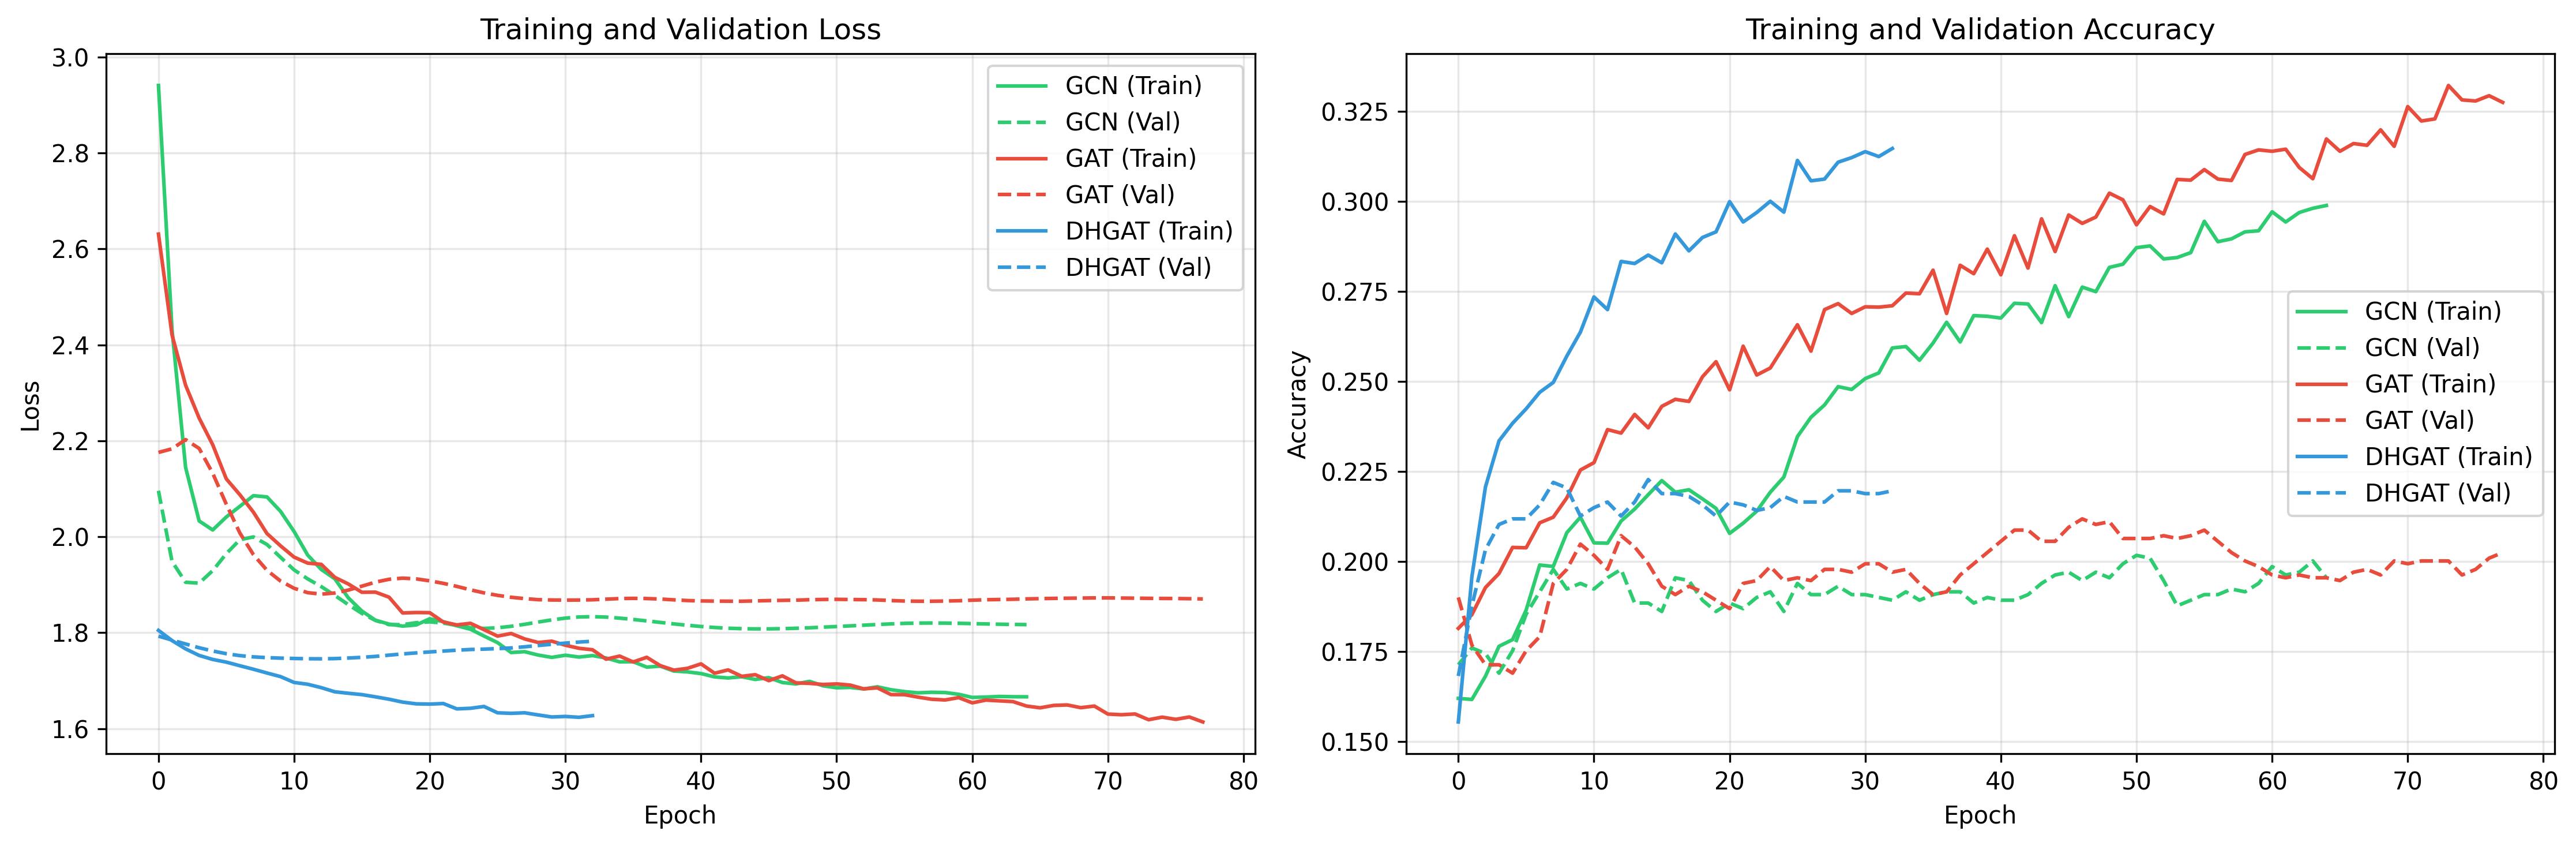
\includegraphics[width=0.85\linewidth]{sections/figures/training_curves.png}
    \caption{Training and validation loss curves for GCN, GAT, and DHGAT models.}
    \label{fig:training_curves}
\end{figure}

Confusion matrices for each model, displayed in Figure~\ref{fig:confusion_matrices}, provide detailed insights into per-class performance.

\begin{figure}[H]
    \centering
    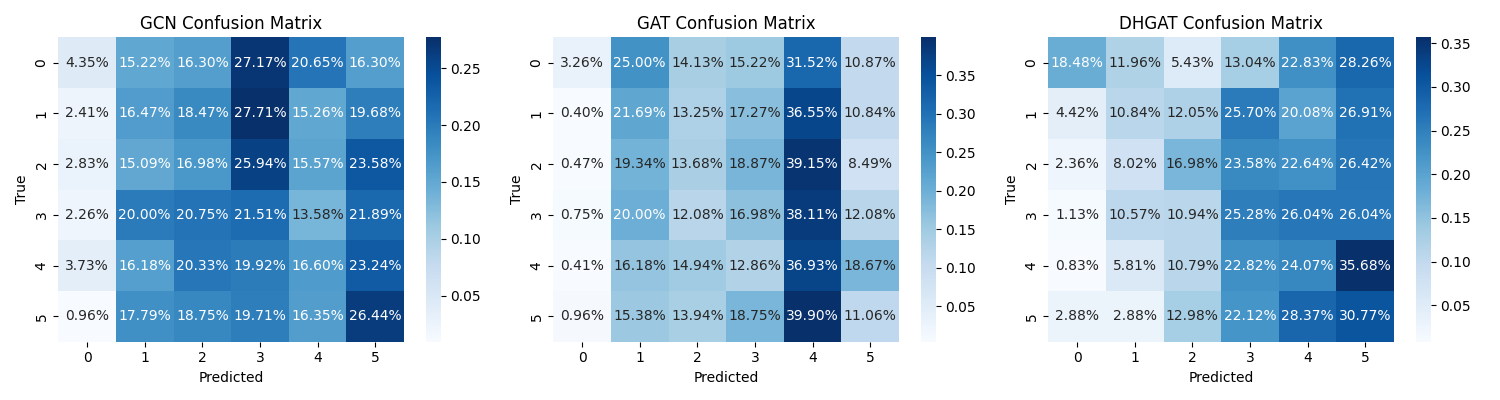
\includegraphics[width=0.95\linewidth]{sections/figures/confusion_matrices.png}
    \caption{Confusion matrices on the test set for GCN, GAT, and DHGAT models.}
    \label{fig:confusion_matrices}
\end{figure}

Finally, Figure~\ref{fig:model_comparison} visualizes the comparative final test accuracies across the three models.

\begin{figure}[H]
    \centering
    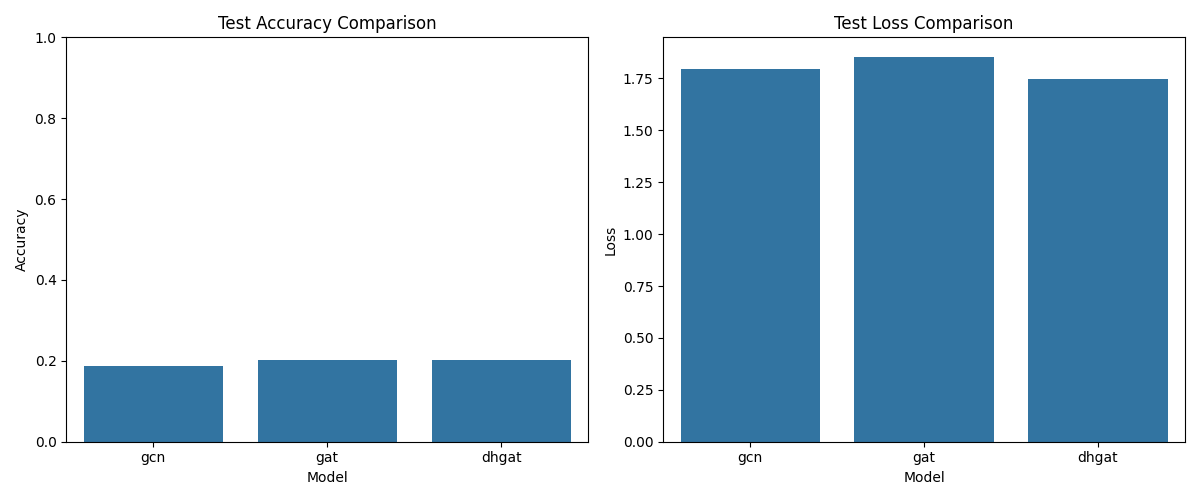
\includegraphics[width=0.7\linewidth]{sections/figures/model_comparison.png}
    \caption{Comparison of final test accuracies across GCN, GAT, and DHGAT models.}
    \label{fig:model_comparison}
\end{figure}

These results suggest that leveraging both content and social relational signals, combined with a dynamic decision mechanism, provides a meaningful advantage for fine-grained fake news classification. Future work may explore extensions toward full heterogeneous graph processing to further enhance relational modeling capabilities.

\section{Critical Analysis}
% Strengths and limitations of your approach
% Learning outcomes: what worked, what didn’t, what you’d do differently
% Value of reproducing vs innovating
\section{Conclusion}
% Summary + future directions

\bibliographystyle{named}
\bibliography{references}

\end{document}
